\chapter{Background}
\label{ch:background}

Some important concepts regarding deep generative models and constrained problems are now presented. They are an essential tool to understand how modern algorithms can be effectively used to solve well-known complex problems. It is out of the scope of this work to discourse on the history of artificial intelligence and deep learning, as well as on any philosophical consideration regarding how technological progress will impact on our lives. The only relevant aspect is that in the last two decades machine learning techniques have experienced a resurgence due to concurrent advances in computational power, availability of large amounts of data and theoretical understanding, becoming an essential part of the technology industry and helping to solve many challenging problems in different fields.

\section{Artificial intelligence}

Today, artificial intelligence (AI) is a thriving multidisciplinary field of research, involving, among the others, computer science, mathematics, psychology, linguistics and philosophy. Despite this, it is difficult to exactly define what AI is, probably due to the lack of a generally accepted \textit{theory of intelligence}, which is an active research topic on its own \cite{machine_intelligence}. Informally, an intelligent machine should be able to mimic human cognitive functions to solve complex problems, such as searching through a large space of solutions, recognizing patterns, learning from experience, using planning methods and reasoning about complex models via induction \cite{steps_towards_AI}. These capabilities seem to be the quintessence of intelligence and are required to solve many real-life problems, such as mechanical translation, game playing, theorem proving and natural language understanding. This is the reason why researchers are concentrating their efforts to study this kind of problems: once solved, they would probably offer solutions applicable to wider areas, such as medical diagnoses. On the other side, as machines become increasingly capable, tasks once considered as requiring intelligence are often removed from the definition, becoming ``simple computation''. This phenomenon is known as the \textit{AI effect} and has lead to the witty Tesler's ``theorem'' \cite{golden_braid}:


\begin{Theorem}
    AI is whatever hasn't been done yet.
\end{Theorem}

In computer science, there is no established unifying theory or paradigm that guides AI research. Some of the approaches include traditional symbolic AI, logic programming and statistical methods, most of them relying on a large number of tools such as probabilistic methods for uncertain reasoning or mathematical optimization.
Several AI projects have tried to hard-code knowledge about the world in formal languages, in order to allow computers to automatically reason about statements using logical inference rules. This is known as the knowledge-base approach to AI. The difficulties faced by these systems suggest that they need the ability to acquire their own knowledge, by extracting patterns from raw data. This capability is known as \textit{machine learning}.


\subsection{Machine learning}

Machine learning (ML) explores the study of algorithms that can automatically learn from examples and then make predictions on new data. It is employed in a wide range of computing tasks where designing and programming explicit algorithms with good performance is difficult or infeasible. Some applications involve, for instance, spam filtering, detection of network intruders, optical character recognition and computer vision.

A formal definition is provided by Mitchell \cite{mitchell}:

\begin{Definition}
    A computer program is said to learn from experience E with respect to some class of tasks T and performance measure P if its performance at tasks in T, as measured by P, improves with experience E.
\end{Definition}

This definition of the tasks in which machine learning is concerned is \textit{operational} and does not involve any cognitive term. It also follows Turing's proposal of focusing on whether machines could \textit{do} what humans can do, acting indistinguishably from them, rather than concentrating on \textit{thinking} in a broader sense \cite{alan}.

ML tasks are typically classified into two broad categories, depending on whether there is a learning feedback available to the systems: \textit{unsupervised} and \textit{supervised learning}. Unsupervised learning is the task of inferring a function to describe hidden structures from unlabelled data, input observations that do not include any explicit information related to the expected output of the algorithm. On the contrary, supervised learning is the task of learning a function that maps an input to an output based on training data consisting of labelled pairs. More formally, the goal of a supervised learning model is to approximate a function $f^* : \mathbb{X} \to \mathbb{Y}$ of interest for the given task, with $\mathbb{X}$ and $\mathbb{Y}$ some generic input and output domains. For instance, in order to build a classifier, a system should try to approximate at its best the function $y=f^*(\bm{x})$ that maps an input $\bm{x}$ to a category $y$. In case of supervised learning tasks, the system will be given training data pairs $(\bm{x}, \bm{y}) \in \mathbb{X} \bigtimes \mathbb{Y}$; in case of unsupervised learning tasks, on the contrary, it will only receive some examples $\bm{x} \in \mathbb{X}$. As special cases, the input signal can be only partially available or restricted to particular feedback. For instance, in \textit{semi-supervised learning} the algorithm is given a training set with some target outputs missing; in \textit{reinforcement learning} training data, in form of rewards and punishments, are given only as feedback to the program's actions in a dynamic environment.

The core objective of a learner is to generalize from its experience \cite{bishop}. Generalization is the ability of a computer program to perform accurately on new, unseen examples or tasks after having experienced a learning data set. Typically, the training examples come from an unknown probability distribution and the learner has to build a general model about this space that enables it to produce sufficiently accurate predictions in new cases.

The performance of ML algorithms heavily depends on the \textit{representation} of the data they are given. This is a general phenomenon that appears throughout computer science and even daily life. To recognize the importance of data representation consider how fast can be searching a collection of data if it has been structured and indexed appropriately or how easy is for people arithmetic on Roman numerals with respect to the one on Arabic numerals. Some tasks can be solved by carefully designing the right set of \textit{features} and then providing these features to simple models. However, in many tasks it is difficult to know in advance which features are more relevant. One solution to this problem is to use ML to discover not only the mapping from representation to output but also the representation itself. This approach is known as \textit{representation learning}. Learnt representations often result in better performances than those obtained with hand-designed representations. Furthermore, they also allow systems to rapidly adapt to new tasks with minimal human intervention. A family of techniques exploiting the idea of automatically finding an appropriate representation of data in order to solve ML tasks is \textit{deep learning}.


\section{Deep learning}

Deep learning (DL) is a class of ML algorithms and techniques that, in recent years, has seen a tremendous growth in popularity and applicability due to some key factors. It has already proven useful in many software disciplines, including computer vision, natural language and audio processing, robotics, bioinformatics, chemistry, video games, search engines, online advertising and finance. The main ideas behind DL have been around for many decades, if not centuries, but they have been effectively applied only in the last few years due to more powerful central processing units (CPUs), general-purpose computing on graphics processing units (GPUs), larger available data sets and clever training techniques. In \cite{The_DL_book}, in fact, the authors point out that the \textit{Age of Big Data} has made ML much easier because the key burden of statistical estimation has been considerably lightened. In addition, this trend is generally expected to continue well into the future.

Modern DL draws inspiration from many fields, especially linear algebra, probability, information theory and numerical optimization. However, neuroscience is regarded as one of the most important sources of inspiration for DL researchers, even if today there is no enough available information about the brain
to use it as a guide. Nevertheless, it is worth noting that understanding how the brain works on an algorithmic level is currently studied in \textit{computational neuroscience}.

DL achieves great power and flexibility by automatically learning the best representation for a given task as a nested hierarchy of concepts, with each concept defined in relation to simpler ones, and more abstract representations computed in terms of less abstract ones. If one draws a graph showing how these concepts are built on top of each other, the result is often a deep stack made up of many layers. For this reason, this family of algorithms is called \textit{deep} learning.

A similar learning mechanism can be observed in human brains, where neurons are connected in a complex network and cooperate to compute some kind of functions. To some extent, they can be considered computational units, each one retaining a piece of information or part of a representation, organized in a meaningful structure. By drawing inspiration from this model, ML researchers have focused their efforts theorizing a mathematical counterpart. The result has been the development of \textit{artificial neural networks}.



\subsection{Artificial neural networks}

An artificial neural network (ANN) is a function $f : \mathbb{X} \to \mathbb{Y}$, with $\mathbb{X}$ and $\mathbb{Y}$ some generic input and output domains. An ANN $f$ is typically defined as a composition of other functions $f^{(1)}$, $f^{(2)}$, ..., $f^{(n)}$. It is precisely due to this composition that they are called \textit{multilayer} networks. Depending on how these functions are composed together, an ANN can be classified as a \textit{feedforward neural network} (FNN) or as a \textit{recurrent neural network} (RNN). In FNNs the functions composition forms directed acyclic graphs, while in RNNs graphs can contain cycles. This work focuses on the former.

\begin{figure}[ht]
    \centering
    \begin{minipage}{0.4\textwidth}
        \centering
        
\includegraphics[width=0.6\textwidth]{fnn_schema}
        \caption{Schematic representation of a feedforward neural network.}
    \end{minipage}
    \hspace{0.5cm}
    \begin{minipage}{0.4\textwidth}
        \centering
        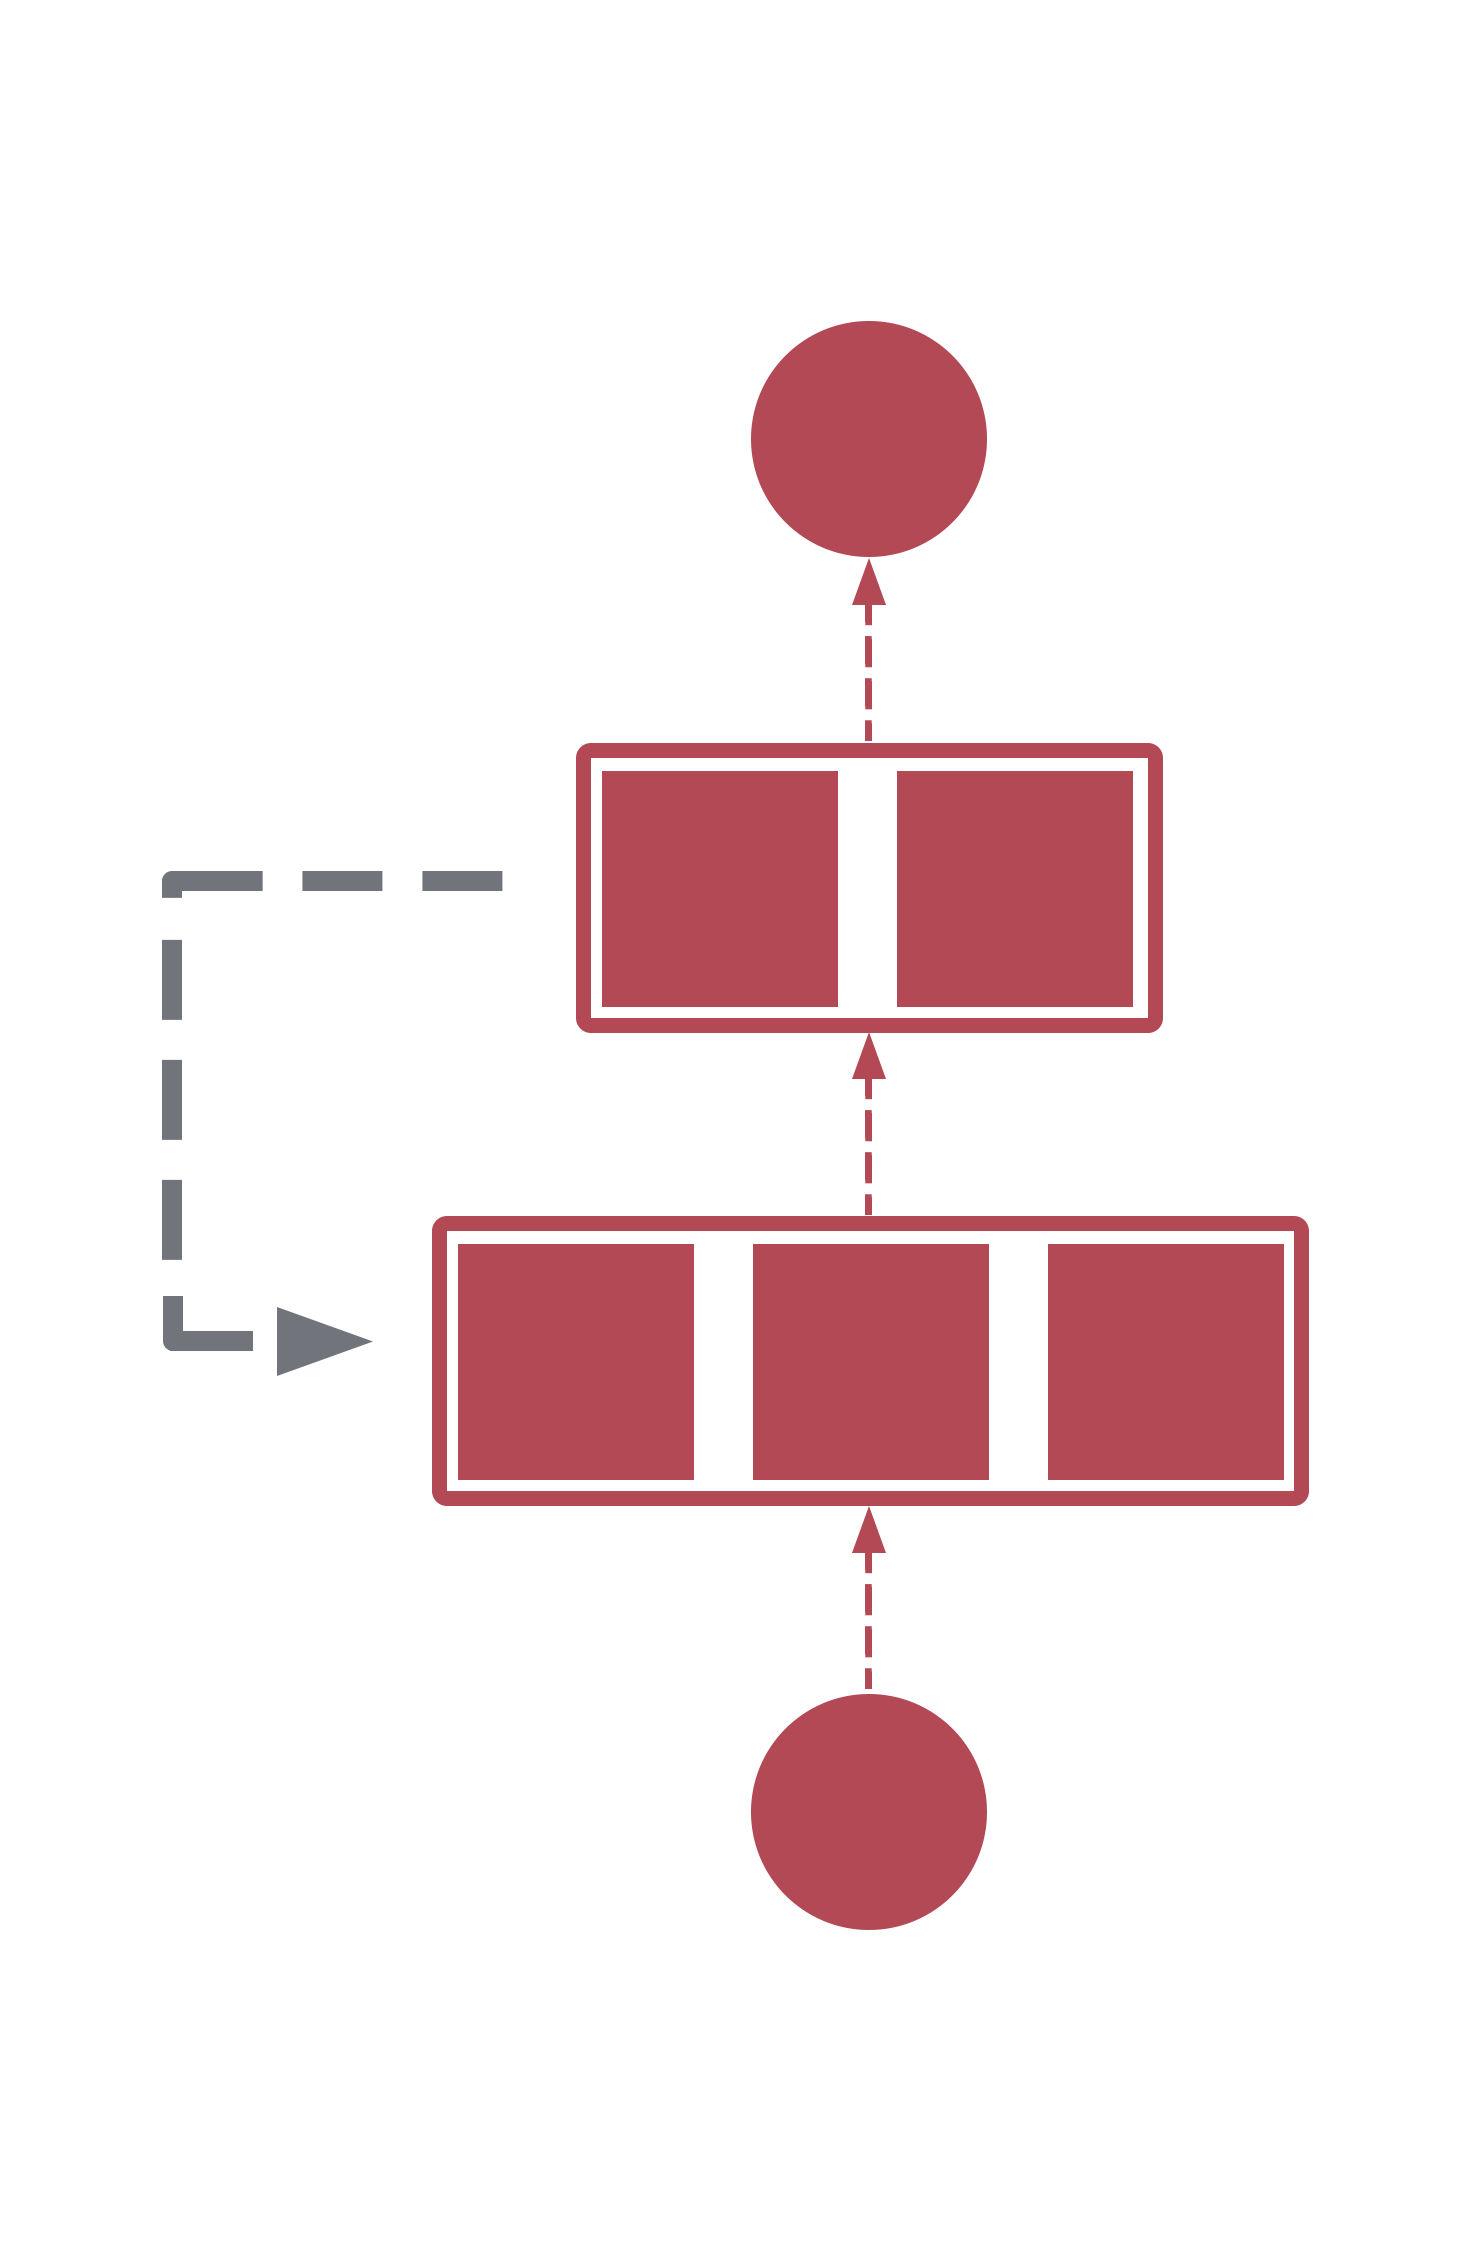
\includegraphics[width=0.6\textwidth]{rnn_schema}
        \caption{Schematic representation of a recurrent neural network.}
    \end{minipage}
\end{figure}

An example of FNN is the function obtained by chaining three components $f^{(1)}$, $f^{(2)}$ and $f^{(3)}$, yielding $f(\bm{x}) = f^{(3)}(f^{(2)}(f^{(1)}(\bm{x})))$. In this case, $f^{(1)}$ is called the \textit{first layer} of the network, $f^{(2)}$ is the \textit{second layer} and $f^{(3)}$, the final layer, is the \textit{output layer}. The overall length of the chain gives the \textit{depth} of the model. Training examples specify directly only what the output layer should return, with no clue on the behaviour of other layers. It is up to the ML algorithm to decide how to use those layers to produce the desired output that approximates $f^*$, the target function to learn, of interest for the given ML task. For this reason, they are called \textit{hidden layers}. 

Hidden layers are usually vector-valued and their dimensionality determines the \textit{width} of the model. Every element of the vector may be interpreted as a human neuron and the layer can be considered as consisting of many \textit{units} that act in parallel, each representing a vector-to-scalar function. Each unit resembles a neuron since it receives inputs from many other connected units (or from the external environment, in case of the first layer) and then computes its own activation value. However, the goal of ANNs is not to perfectly model the brain, even though the choice of the some layer functions $f^{(i)}$ is sometimes guided by neuroscientific observations on biological neurons.

ML tasks often require to learn a nonlinear function $f^*$. In order to compute a nonlinear function of $\bm{x}$ at least one layer $f^{(i)}$ of the ANN must involve a nonlinear transformation, otherwise the final output of the network would remain a linear combination of its intermediate results. Most FNNs rely on an affine transformation on every hidden layer, followed by a fixed nonlinear function called \textit{activation function}. The output layer, on the contrary, does not usually apply any further nonlinear transformation. As a result, every hidden layer consists of a vector of hidden units $\bm{h}^{(i)}$ computed by the corresponding nonlinear function $f^{(i)}(\bm{x}; \bm{W}^{(i)}, \bm{c}^{(i)})$, where $\bm{W}^{(i)}$ provides the weights of the linear transformation and $\bm{c}^{(i)}$ the biases. The network thus computes the values of some hidden units and then uses them as input for the next layer. By doing so, information flows in a unidirectional way from one hidden layer to the next, up to the output layer. This is the reason why this kind of neural network is called feedforward.

The computational process of a FNN just described can be now formally defined. Given a FNN $f : \mathbb{X} \to \mathbb{Y}$ composed by $n$ functions (layers) $f^{(1)}$, $f^{(2)}$, ..., $f^{(n-1)}$, $f^{(n)}$, we have

\begin{equation}
\label{eq:ANN_compact}
f(\bm{x}) = f^{(n)}(f^{(n-1)}(...(f^{(2)}(f^{(1)}(\bm{x}))))),
\end{equation}

where
\begin{equation}
\label{eq:ANN_layers}
f^{(i)}(\bm{x}) =
\begin{cases}
    g^{(i)}(\bm{W}^{(i)\top} \bm{x} + \bm{c}^{(i)}) & \text{if i} = 1\\
    g^{(i)}(\bm{W}^{(i)\top} f^{(i-1)}(\bm{x}) + \bm{c}^{(i)}) & \text{otherwise}
\end{cases},
\end{equation}

with $g^{(i)}$ arbitrary activation functions, $\bm{W}^{(i)}$ layers weights and $\bm{c}^{(i)}$ layers biases.

For convenience, all these parameters are usually grouped in a vector $\bm{\theta}$. Training an ANN amounts to finding a $\bm{\theta}$ such that   $f(\bm{x}; \bm{\theta})$ well approximate $f^*(\bm{x})$. This is usually done with information provided by a \textit{loss function}.



\subsection{Loss functions}

In mathematical optimization, a loss function $l : \mathbb{A} \to \mathbb{R}$ assigns a cost to an event or value. This number intuitively measures how bad the effects of an event are or how distant is the input value from the target one. An optimization problem obviously seeks to minimize the loss function. In some cases, the objective function is the opposite of $l$, it is called \textit{reward function}, and the equivalent goal is to maximize it.

The loss functions of ANNs are similar to those of other parametric models. In most cases, a network defines a distribution $p(\bm{y} | \bm{x}; \bm{\theta})$, so it is possible to estimate $\bm{\theta}$ via \textit{maximum likelihood estimation}, a popular method of estimating statistical model parameters given observations. 

ANNs are thus often trained using the cross entropy between the empirical distribution defined by the training set $\hat{p}_{data}$ and the model distribution $p_{model}$:

\begin{equation}
l(\bm{\theta}) = - \mathbb{E}_{\bm{x}, \bm{y} \sim \hat{p}_{data}} \log p_{model}(\bm{y}|\bm{x}),
\end{equation}

where $l$ is the loss function associated to the entire network.

An advantage of deriving the loss function from maximum likelihood is that it removes the burden of designing a new loss function for each model: specifying a model $p_{model}(\bm{y} | \bm{x})$ automatically determines a cost function $\log p_{model}(\bm{y} | \bm{x})$.

Regardless of which loss function is chosen to train the model, the minimization of the error is achieved through an optimization method, such as \textit{gradient descent}. For such reason, the loss function must be differentiable. In addition, in order to serve as a good guide throughout all the training algorithm, its gradient should always be large and predictable. Functions that saturate undermine this objective because they produce very small gradients. In many cases
this happens because the activation functions used to compute the output of the hidden units or the output units saturate. The logarithm in the negative log-likelihood loss function succeeds in undoing the problematic effect caused by output units involving exponential functions that saturate when their argument is very small.

Error minimization through gradient descent \cite{hadamard1908memoire} in the parameters space of
complex, nonlinear, differentiable systems has been discussed at least since the early 1960s, initially within the framework of Euler-Lagrange equations in the calculus of variations \cite{Euler:1744}. However, an efficient procedure to minimize loss functions was first described only a decade later \cite{Linnainmaa:1970}\cite{Linnainmaa:1976}, with the design of the algorithm of \textit{backpropagation}.



\subsection{Backpropagation}

Backpropagation is an efficient method used during ANNs training to compute how weights connecting units should be updated with respect to the value of the loss function.
The systems of the 1960s transmitted derivative information through standard Jacobian matrix calculations from one ``layer'' to the previous one, without explicitly addressing either direct links across several layers or potential additional efficiency gains due to network sparsity, typical of ANNs.
Modern backpropagation overcomes these limitations with a computational cost essentially equivalent of the forward pass.

Equations \eqref{eq:ANN_compact} and \eqref{eq:ANN_layers} concisely describe how ANNs layers as a whole interact with each other. However, to easily describe the backpropagation algorithm, it is handy to define some additional ones that involve single units.

We define $w_{i,j}$ as the weight connecting two units $h_i$ and $h_j$ belonging to different layers. $\mathbb{W}$ is the set of such weights. An iterative optimization algorithm should try to optimize each $w_{i,j}$, step by step, according to the error measured by $l$. This is done with gradient descent in the following way:

\begin{equation}
w_{i,j} \gets w_{i,j} - \eta \frac{\partial l}{\partial w_{i,j}},
\end{equation}

where $\eta \in \mathbb{R}$ is the \textit{learning rate}.

We define $pred_j$ as the set of input units connected to $h_j$:

\[
pred_j = \{h_i | w_{i,j} \in \mathbb{W} \}
\]

and, similarly, $succ_j$ as the set of output units connected to $h_j$:

\[
succ_j = \{h_i | w_{j,i} \in \mathbb{W} \}
\]

Supposing a fixed differentiable activation function $\varphi$ for every unit, we define $net_j$ as the input $h_j$ receives from the units it is connected to:

\[
net_j = \sum\limits_{k}^{pred_j} w_{k,j} \cdot o_k,
\]

where $o_k = \varphi(net_k)$ is the output of $h_k$. If the unit $h_k$ is in the first layer after the input layer, than $o_k$ is just $\bm{x}_k$, with $\bm{x}$ being a training example.

Each weight $w_{i,j}$ should be updated according to:

\begin{equation}
\label{eq:bp_final}
\frac{\partial l}{\partial w_{i,j}} = \delta_j \cdot o_i,
\end{equation}

where
\[
\delta_j =
\begin{cases}
     \frac{\partial l}{\partial f(\bm{x}_j)} \cdot \varphi\prime(net_j) & \text{if unit $h_j$ in output layer} \\ \\
     \sum\limits_{k}^{succ_j} \delta_k \cdot w_{j,k} \cdot \varphi\prime(net_j) & \text{otherwise}
\end{cases}.
\]

The full derivation of \eqref{eq:bp_final} can be found in appendix \ref{sec:appendix_backprop}.

The resulting iterative procedure to train an ANN via gradient descent is described by algorithm \ref{alg:gradient_descent}.

\begin{algorithm}
\caption{Gradient descent algorithm to train an ANN}
\label{alg:gradient_descent}
\begin{algorithmic}[1]
\Require ANN $f$
\Require initialized set of weights $\mathbb{W}$
\Require loss function $l$
\Require learning rate $\eta$
\While {the stopping criterion is not satisfied} \label{line:criterion}
    \ForAll {training examples $(\bm{x}, \hat{\bm{y}})$} \label{line:x_loop}
        \State $\bm{y} \gets f(\bm{x})$
        \Comment compute ANN output
        \ForAll {weight $w_{i,j} \in \mathbb{W}$}
            \State $\Delta w_{i,j} \gets \delta_j \cdot \bm{y}_i$ 
            \Comment see equation \eqref{eq:bp_final} 
            \State $w_{i,j} \gets w_{i,j} - \eta \Delta w_{i,j}$
            \Comment update weight according to loss
        \EndFor
    \EndFor
\EndWhile
\end{algorithmic}
\end{algorithm}

During the initialization phase, weights are usually given small random values. The stopping criterion (line \ref{line:criterion}) can be any predicate reasonable for the learning task, such as \textit{all training examples are classified correctly} or \textit{the error computed by the loss function $l$ is below a given threshold}. This procedure is usually repeated several times; the number of times training examples are used once to update the weights is an \textit{epoch}.

Many widely adopted techniques in DL are discovered empirically and systematically applied because they work well in practice, even if their theoretical background is still uncertain and sometimes it happens to see little algorithmic tricks that effectively improve the overall performances of the ANNs. In the same way, it is also common to see approximations that make computation faster or even feasible, without a significant loss in performance. For instance, the gradient descent algorithm is usually modified to process little groups of training examples, called \textit{mini-batches}, instead of one example at a time (line \ref{line:x_loop}) or by randomly shuffling the training set at each new iteration (line \ref{line:criterion}), giving rise to the \textit{stochastic gradient descent algorithm} (algorithm \ref{alg:stochastic_gradient_descent}). It is now worth pointing out some other theoretical considerations.

\begin{algorithm}
\caption{Stochastic gradient descent algorithm to train an ANN}
\label{alg:stochastic_gradient_descent}
\begin{algorithmic}[1]
\Require ANN $f$
\Require initialized set of weights $\mathbb{W}$
\Require loss function $l$
\Require learning rate $\eta$
\Require mini-batch size $m$
\While {the stopping criterion is not satisfied}
    \State $mb \gets$ data mini-batch \{$(\bm{x}^{(1)}, \hat{\bm{y}}^{(1)})$, $(\bm{x}^{(2)}, \hat{\bm{y}}^{(2)})$, ..., $(\bm{x}^{(m)}, \hat{\bm{y}}^{(m)})$\} randomly sampled from training set 
    \For{$k \gets 1, m$}
        \State $\bm{y}^{(k)} \gets f(mb_k[\bm{x}])$
        \Comment compute ANN outputs
    \EndFor
    \ForAll {weight $w_{i,j} \in \mathbb{W}$}
        \State $\Delta w_{i,j} \gets 0$
        \For{$k \gets 1, m$}
        \State $\bm{x} \gets mb_k[\bm{x}]$
        \State $\bm{y} \gets \bm{y}^{(k)}$
            \State $\Delta w_{i,j} \gets \Delta w_{i,j} + \delta_j \cdot \bm{y}_i$ 
            \Comment see equation \eqref{eq:bp_final}
        \EndFor
        \State $w_{i,j} \gets w_{i,j} - \eta \cdot \frac{1}{m} \cdot \Delta w_{i,j}$
        \Comment update weight according to average loss
    \EndFor
\EndWhile
\end{algorithmic}
\end{algorithm}


\subsection{Theoretical considerations}

A number of considerations about DL should be kept in mind when designing ANNs.

First of all, the \textit{``no free lunch'' theorem} for ML \cite{nfl} states that, averaged over all possible data generating distributions, every classification algorithm has the same error rate when classifying previously unobserved examples. In other words, no ML algorithm is universally any better than any other. However, the goal of ML research is not to seek a universal learning algorithm, but to design systems that perform well on specific tasks. For such reason, there is no need to average over all possible data distributions, since only a tiny subset of them are relevant for the real world we experience. The theorem suggests that ML algorithms should be developed by encoding a set of preferences into the learning algorithm itself. If this is done appropriately, than the algorithm will solve the task it is designed for.

Secondly, the central challenge in ML is generalization. The generalization error of a ML model is typically estimated by measuring its performance on a test set of examples unavailable during training. The factors determining how well a ML algorithm will perform are its abilities to make both the training error and its gap with the test error small. These two factors correspond to two known problems in ML: \textit{underfitting} and \textit{overfitting}. The former occurs when the model is not able to obtain a sufficiently low error value on the training set, the latter when the gap between the training error and the test error is too large. One can control whether a model is more likely to overfit or underfit by altering its \textit{capacity}, the ability to fit a wide variety of functions. What should be kept in mind is that, typically, as model capacity increases, training error decreases until it asymptotes to the minimum possible value, while generalization error has a U-shaped curve and, after a certain point, it will start increasing. With \textit{regularization} it is possible to reduce the generalization error without any impact on the training error.


\begin{figure}[ht]
\centering
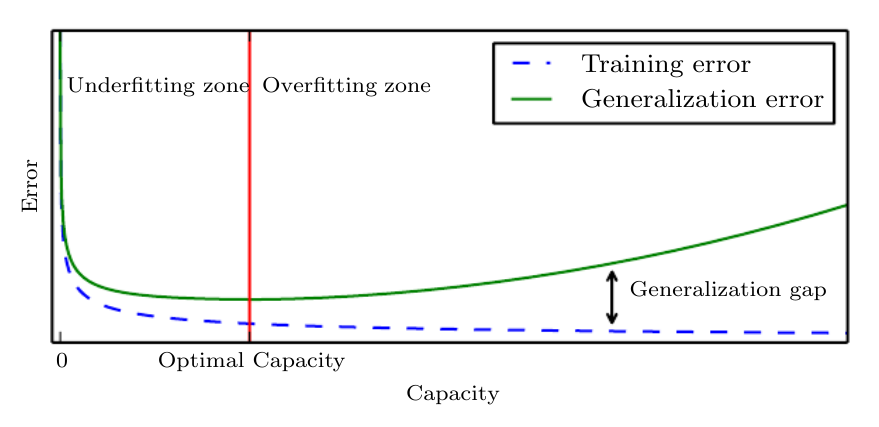
\includegraphics[width=0.8\textwidth,keepaspectratio]{errors}
\caption{Typical relationship between capacity and error as illustrated in \cite{The_DL_book}. At the left end of the graph, training error and generalization error are both high, in the underfitting regime. As capacity increases, training error decreases, but the gap between training and generalization error increases. Eventually, the size of this gap outweighs the decrease in training error and overfitting regime is reached.}
\end{figure}


A final considerations regards \textit{hyperparameters}, a set of values defining higher level concepts about the model, such as the network learning rate. Since they cannot be learnt directly from the training data, they are usually empirically found by testing different models on a validation set, another set of data unavailable during training, and then selecting the best ones. Hyperparameters tuning can be expensive and is an active research field since these values can largely impact on the final performance of the network.
% TODO ref




\section{Deep generative models}


ML models are typically divided into two complementary classes: \textit{discriminative models} and \textit{generative models}. From a probabilistic point of view, discriminative methods try to learn a mapping from input variables $x$ to output variables $y$ directly modelling the conditional probability distribution $p(y|x)$. On the contrary, generative methods try to learn the joint probability distribution $p(x, y)$ underlying the data. Since $p(x, y)$ can be used to compute $p(y|x)$, generative models can also be used to make predictions. However, probably due to the easier nature of their goal, discriminative algorithms often achieve better results in classification tasks and are generally preferred \cite{disc_vs_gen}. Nevertheless, generative models are actively studied because of their peculiar capability of generating new data resembling those in input once $p(x, y)$ is learnt.

Some generative models allow the probability distribution function to be evaluated explicitly, while others only support operations that implicitly require knowledge of it, such as sampling. Techniques to automatically learn an approximation of the real data distribution are particularly useful when learning the exact one is hard or even impossible. Indeed, modern generative networks, when given enough training examples and capacity, often succeed in learning a distribution very similar to the true one. The key insight is that ANNs used for generative models are forced to learn representations in a space significantly smaller than the one of training data and so they are forced to learn meaningful features in order to later generate new data.

\begin{figure}[ht]
\centering
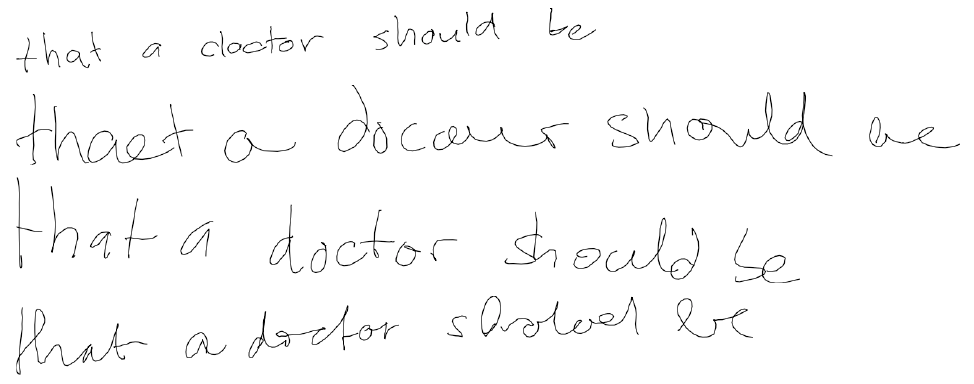
\includegraphics[width=0.8\textwidth,keepaspectratio]{handwritten}
\caption{Different examples of the words sequence ``that a doctor should be'' drawn from a RNN generator \cite{handwritten_rnn}.}
\end{figure}

It is likely that in the near future ANNs will be able to generate samples depicting entirely plausible images or videos. This may by itself find use in multiple applications, such as on-demand generated art \cite{igan} \cite{furniture} (see figure \ref{fig:art_on_demand}). However, one important application of these networks is the generation of synthetic data to augment real data sets, especially for pre-training, a procedure during which the model is trained in advance on data similar to those of the task to avoid random network parameters initialization.
% Nevertheless, it is worth pointing out that no model will ever be able \todor{to generate examples of things it has never seen real examples of before}{troppo generico, non accurato}.
Besides these speculations, present known applications include image denoising, inpainting \cite{inpainting}, super-resolution \cite{growing_gans} \cite{super_gans}, exploration in reinforcement learning and neural network pre-training in cases where labelled data are expensive.

\begin{figure}[ht]
    \centering
    \begin{minipage}{0.32\textwidth}
        \centering
        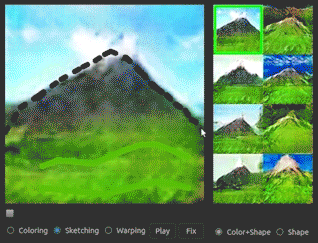
\includegraphics[width=\textwidth]{igan1}
    \end{minipage}
    \begin{minipage}{0.32\textwidth}
        \centering
        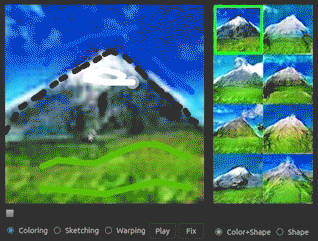
\includegraphics[width=\textwidth]{igan2}
    \end{minipage}
    \begin{minipage}{0.32\textwidth}
        \centering
        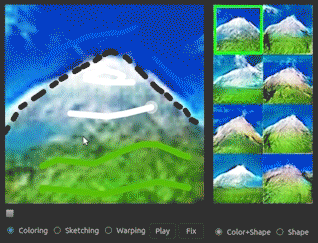
\includegraphics[width=\textwidth]{igan3}
    \end{minipage}
    \caption{Example of interactive image generation from \cite{igan}. A system can produce photo-realistic samples that best satisfy the user edits in real-time.}
    \label{fig:art_on_demand}
\end{figure}


This work focuses on a family of generative models called \textit{generative adversarial networks}.


\subsection{Generative adversarial networks}


% "Adversarial training is the coolest thing since sliced bread." - Yann LeCun, Director of AI Research at Facebook and Professor at NYU

Generative adversarial networks (GANs) are based on a game theoretic scenario in which two networks, a \textit{discriminator} and a \textit{generator}, compete against each other. The goal of the generator is to produce objects similar to the training examples and trick the discriminator into believing they are real. This model can be thus thought as a game between a counterfeiter, trying to produce fake currency, and a policeman, trying to detect it. The idea to infer models in a competitive setting was first used for behavioural inference in the field of ethology \cite{controlled_interaction} and to find binary factorial codes \cite{factorial_codes}.

Formally, we define the discriminator as a network $D(\bm{x}; \bm{\theta}^{(d)})$ and the generator as a network $G(\bm{z}; \bm{\theta}^{(g)})$, where $\bm{z}$ is a random input noise drawn from a distribution $p_z$. We define the generator's probability distributions over data $\bm{x}$ as as $p_g$.

The output of the generator $\bm{x}=G(\bm{z})$ represents a generated object that should resemble those of the training set, while the output of the discriminator $y=D(\bm{x})$ represents the probability that $\bm{x}$ was sampled from $p_{data}$ rather than $p_g$.

The goal of the model is to train simultaneously $D$ and $G$: the discriminator should try to maximize its output probabilities for training examples; the generator should try minimize the probability of generating objects that will be rejected by $D$ (i.e. those receiving a low score). So, $D$ and $G$ play the following minimax game with \textit{value function} $V(D, G)$:

\begin{equation}
\min_G \max_D V(D, G).
\end{equation} 

A typical choice for $V(D, G)$ is

\begin{equation}
V(D, G) = \underbrace{\mathbb{E}_{\bm{x} \sim p_{data}} [\log D(\bm{x})]}_\textrm{\textit{D} goal} + \underbrace{\mathbb{E}_{\bm{z} \sim p_z} [\log (1 - D(G(\bm{z})))]}_\textrm{\textit{G} goal}.
\end{equation}

However, when $G$ has not learnt yet how to produce good objects, $D$ can reject samples from $p_g$ with high confidence. In this case $\log (1 - D(G(\bm{z})))$ saturates, preventing learning. To avoid this issue, $G$ can be instead trained to maximize the opposite function, $\log D(G(\bm{z}))$. Although mathematically equivalent, the second formulation provides better gradients in early training.

\begin{figure}[ht]
    \centering
    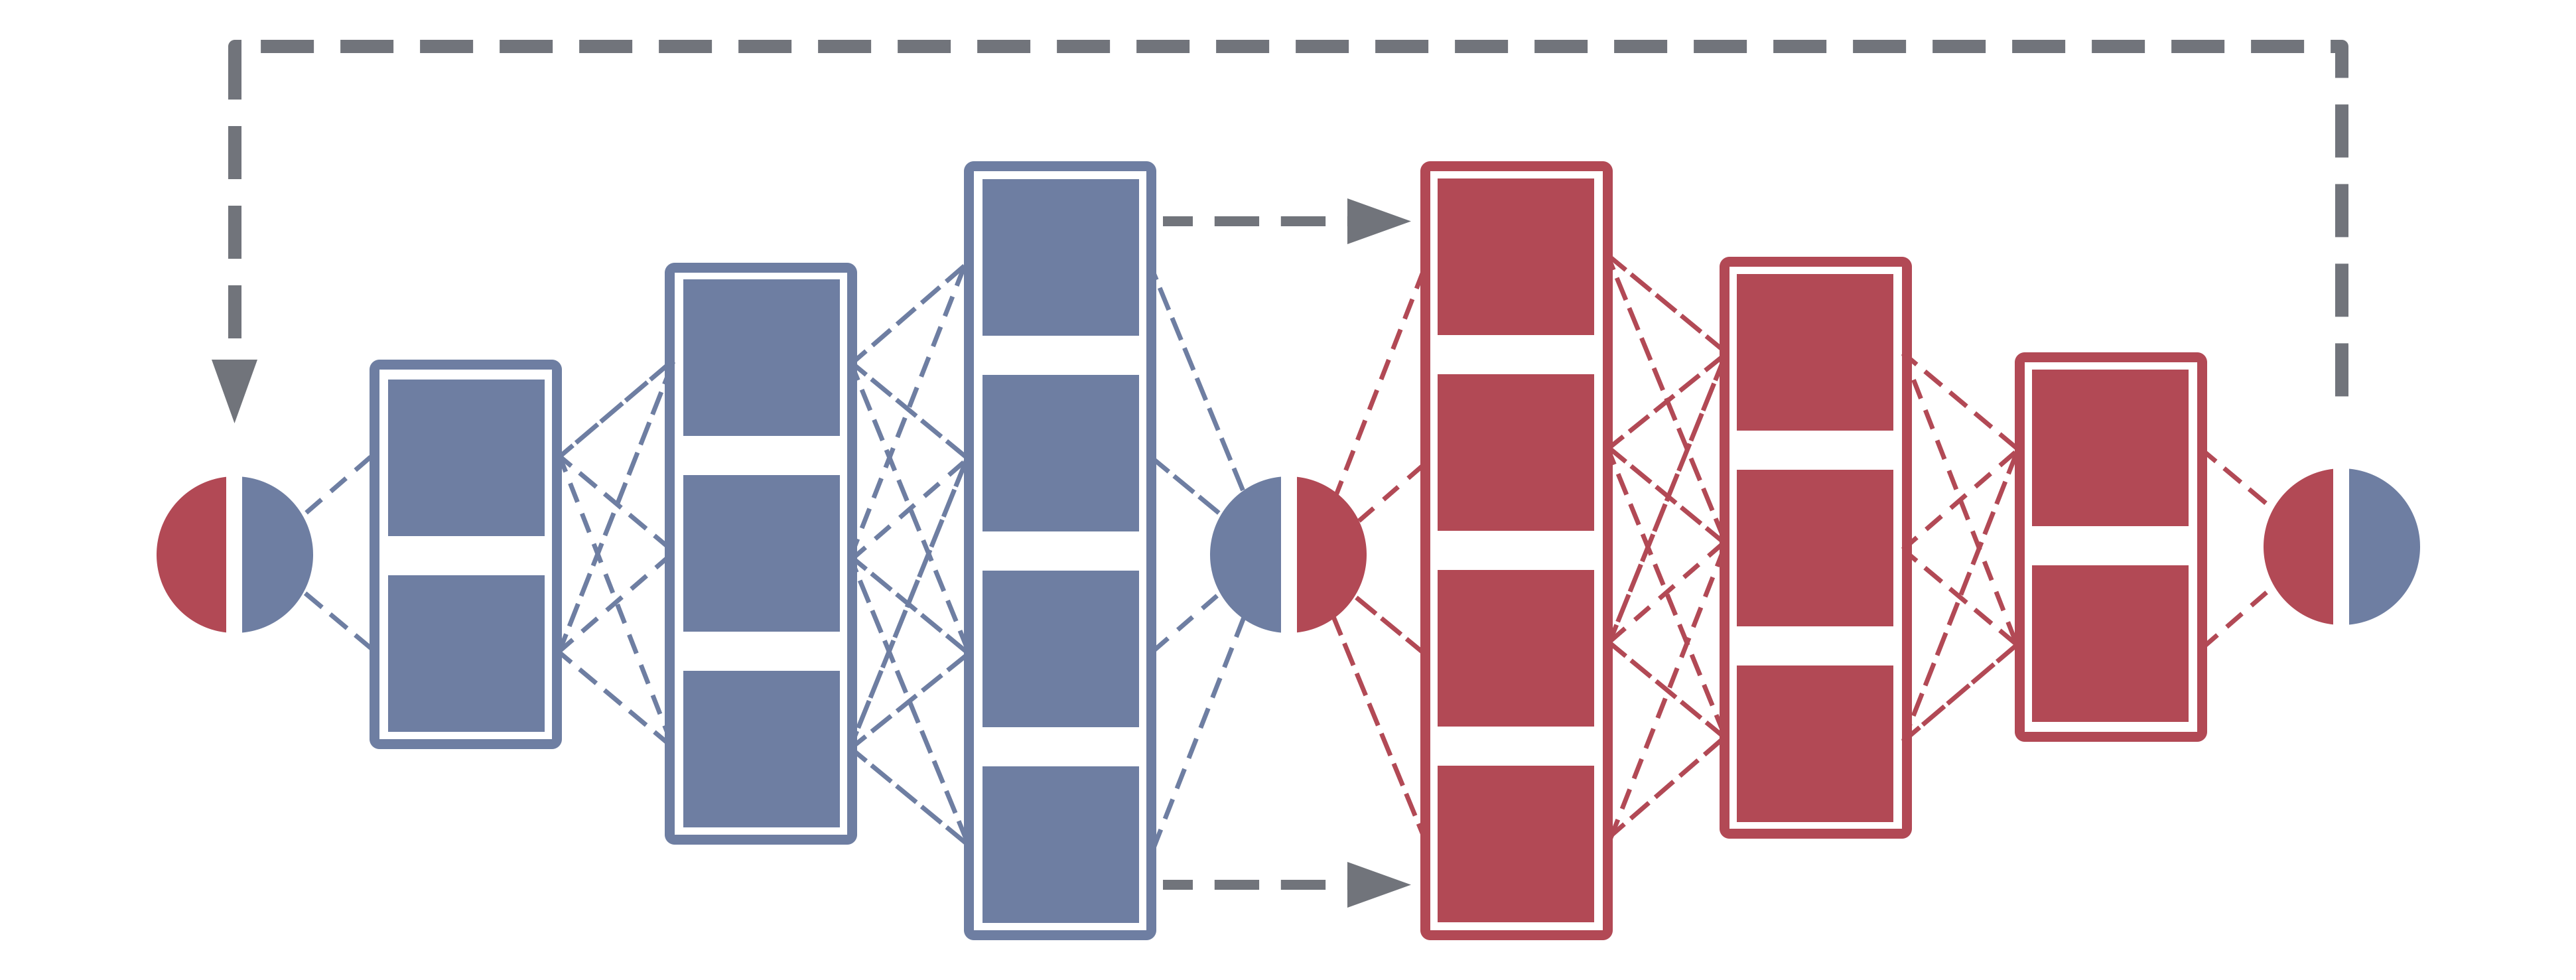
\includegraphics[width=0.7\textwidth]{gan_schema}
    \caption{Schematic representation of GANs with a generator (blue) producing objects for the discriminator (red).}
\end{figure}

In practice, $D$ and $G$ are trained via traditional backpropagation using an iterative approach consisting of two alternating loops of $k$ steps of $D$ optimization and one step of $G$ optimization. This results in $D$ being maintained near its optimal solution as long as $G$ changes slowly enough. Algorithm \ref{alg:sgd_gans} shows the mini-batch stochastic gradient descent training procedure for GANs.

\begin{algorithm}
\caption{Stochastic gradient descent algorithm to train GANs}
\label{alg:sgd_gans}
\begin{algorithmic}[1]
\Require ANN discriminator $D$
\Require ANN generator $G$
\Require discriminator parameters $\bm{\theta}^{(d)}$
\Require generator parameters $\bm{\theta}^{(g)}$
\Require learning rate $\eta$
\Require mini-batch size $m$
\Require discriminator training steps number $k$
\While {the stopping criterion is not satisfied}
    \For {$k$ steps}
        \State $z\_mb \gets$ noise mini-batch \{$\bm{z}^{(1)}$, $\bm{z}^{(2)}$, ..., $\bm{z}^{(m)}$\} randomly sampled from $p_z$
        \State $mb \gets$ data mini-batch \{$\bm{x}^{(1)}$, $\bm{x}^{(2)}$, ..., $\bm{x}^{(m)}$\} randomly sampled from $p_{data}$
        \State $\Delta \bm{\theta}^{(d)} \gets \nabla_{\bm{\theta}^{(d)}} \frac{1}{m} \sum\limits_{i=1}^m [\log D(mb_i) + \log (1 - D(G(z\_mb_i)))]$
        \Comment compute gradient
        \State $\bm{\theta}^{(d)} \gets \bm{\theta}^{(d)} + \eta \Delta \bm{\theta}^{(d)}$ 
        \Comment update D by ascending gradient
    \EndFor
    \State $z\_mb \gets$ noise mini-batch \{$\bm{z}^{(1)}$, $\bm{z}^{(2)}$, ..., $\bm{z}^{(m)}$\} randomly sampled from $p_z$
    \State $\Delta \bm{\theta}^{(g)} \gets \nabla_{\bm{\theta}^{(g)}} \frac{1}{m} \sum\limits_{i=1}^m [\log (1 - D(G(z\_mb_i)))]$
    \Comment compute gradient
    \State $\bm{\theta}^{(g)} \gets \bm{\theta}^{(g)} - \eta \Delta \bm{\theta}^{(g)}$ 
    \Comment update G by descending gradient
\EndWhile
\end{algorithmic}
\end{algorithm}


In a scenario in which the two networks have access to infinite examples, after several training steps, if $G$ and $D$ have enough capacity, they will reach a point at which both cannot improve because $p_g = p_{data}$. In this situation the discriminator will be unable to differentiate between the two distributions and every example will have the same probability of being real or generated, i.e. $D(\bm{x}) = \frac{1}{2}$. In general, given a fixed generator $G$, the optimal discriminator is

\begin{equation}
\label{perfect_gans_D}
D^*_G(\bm{x}) = \frac{p_{data}(\bm{x})}{p_{data}(\bm{x}) + p_g(\bm{x})}
\end{equation}

The main motivation for the design of GANs is that the learning process
requires neither approximate inference nor approximation of a partition function gradient, but only traditional backpropagation. Furthermore, the model is very flexible since $D$ and $G$ can be any ANN and eliminates the need of Markov chains.

On the other side, GANs do not offer an explicit representation of $p_g$. Furthermore, some critical issues may be hidden in the training procedure. First, $D$ and $G$ must be synchronized well in order to avoid the scenario in which the generator collapses too many values of $\bm{z}$ to the same value of $\bm{x}$. This usually happens when $G$ is trained too much, without updating $D$. Second, simultaneous gradient descent in the adversarial game setting is not guaranteed to reach an equilibrium. In fact, it is possible for the two players to take infinite turns increasing and then decreasing the value function forever, rather than landing exactly on the saddle point of $V$ where they cannot further reduce their costs. Note that the equilibria for a minimax game are not local minima of $V$, but saddle points which are local minima with respect to the first player’s parameters and local maxima with respect to the second player’s parameters. Finally, GANs framework is designed for fully differentiable networks $D$ and $G$. This is problematic since many important real-world data sets, such as word-base representations of language, are discrete. However, there exist variants that can deal with discrete variables, such as \textit{boundary-seeking generative adversarial networks}.



\subsection{Boundary-seeking generative adversarial networks}

Boundary-seeking generative adversarial networks (BGANs) provide a unified framework to deal with discrete and continuous variables. For the present work, only the former are of interest and will be further analysed.

Given a fixed generator $G$, from equation \eqref{perfect_gans_D} it is possible to derive the density of data:

\begin{equation}
p_{data}(\bm{x}) = p_g(\bm{x}) \frac{D^*_G(\bm{x})}{1 - D^*_G(\bm{x})}.
\end{equation}

This indicates that, in the limit of a perfect discriminator $D^*$, the true data distribution can be perfectly estimated from such discriminator and any fixed generator $G$, even if that generator is not perfectly trained. A sample from the correct data distribution can thus be obtained by simply reweighing samples drawn from the imperfect distribution $p_g$ according the ratio $\frac{D^*_G(\bm{x})}{1 - D^*_G(\bm{x})}$.

Unfortunately, it is unlikely that the perfect discriminator $D^*$ can be learnt or even exists. However, given an imperfect discriminator $D$, the true data distribution $p_{data}$ can be approximated in the following way:

\begin{equation}
\label{eq:p_data_estimator}
\widetilde{p}_{data}(\bm{x}) = \frac{1}{Z} p_g(\bm{x}) \frac{D(\bm{x})}{1 - D(\bm{x})},
\end{equation}

where

\[
Z = \sum\limits_{\bm{x}} p_g(\bm{x}) \frac{D(\bm{x})}{1 - D(\bm{x})}
\]

is the normalization constant that guarantees $\widetilde{p}_{data}$ to be a proper probability distribution. The bias $\widetilde{p}_{data}$ is affected to only depends on the quality of $D$: the closer $D$ is to $D^*$, the lower the bias. This is a nice property, since training the discriminator (a standard probabilistic binary classifier) is generally easier than training the generator (whose objective function is a moving target as the discriminator adapts to the generator and vice versa). Note that the optimum for the generator occurs at $D(\bm{x}) = D^*(\bm{x}) = \frac{1}{2}$, so that $Z = 1$ and $p_{data} = \widetilde{p}_{data} = p_g$. This occurs at the decision boundary of the discriminator, when generated samples have the same probability of being classified as real data or samples. This is the reason for the name BGANs.

GANs have serious limitations on the type of variables they can model, because they require the composition of the generator and discriminator to be fully differentiable. With discrete variables this is not true. For instance, consider using a step function at the end of a generator in order to generate a discrete value. In this case, backpropagation alone cannot provide the training signal for the generator, since the derivative of a step function is $0$ almost everywhere and so would be the backpropagated signal. The goal of BGANs is to train a generator outputting discrete values by estimating gradients for $\bm{\theta}^{(g)}$ via the exclusive Kullback-Leibler divergence between the two joint distributions $p_{data}(\bm{x}, \bm{z})$ and $p_g(\bm{x}, \bm{z})$:

\begin{equation}
\nabla_{\bm{\theta}^{(g)}} D_{KL}(p_{data}(\bm{x}, \bm{z}) || p_g(\bm{x}, \bm{z})),
\end{equation}

or by using the biased estimator:

\begin{equation}
\label{eq:dkl_bgans}
\nabla_{\bm{\theta}^{(g)}} D_{KL}(\widetilde{p}_{data}(\bm{x}, \bm{z}) || p_g(\bm{x}, \bm{z})).
\end{equation}

The generator distribution $p_g(\bm{x})$ can be parametrized as the marginalization of a joint density
\begin{equation}
\label{eq:cond_prob_g}
p_g(\bm{x}) = \sum\limits_{\bm{z}} g(\bm{x}|\bm{z})p_z(\bm{z}), 
\end{equation}

where $g(\bm{x}|\bm{z})$ is the conditional distribution of the generator function.

The result of the computation of the gradient in equation \eqref{eq:dkl_bgans} is:

\begin{equation}
\label{eq:gradient_bgans}
\nabla_{\bm{\theta}^{(g)}} D_{KL}(\widetilde{p}_{data}(\bm{x}, \bm{z}) || p_g(\bm{x}, \bm{z})) \approx - \mathbb{E}_{\bm{z} \sim p_z(\bm{z})} [\sum\limits_{m = 1}^{M} \widetilde{w}^{(m)} \nabla_{\bm{\theta}^{(g)}} \log g(\bm{x}^{(m)} | \bm{z})],
\end{equation}

where
\[
\widetilde{w}^{(m)} = \frac{w^{(m)}}{\sum\limits_{m'} w^{(m')}} 
\]

and

\[
w^{(m)} = \frac{D(\bm{x}^{(m)})}{1 - D(\bm{x}^{(m)})} 
\]

are the normalized and unnormalized importance weights and $\bm{x}^{(m)}$ are samples from the generator for the given $\bm{z}$. The normalization can help to generate a relative learning signal that is particularly useful when samples are all fairly bad from the point of view of $D(\bm{x})$.

% TODO spiegare meglio la questione dei valori discreti. Guarda intro BGAN

This allows to compute gradients from a mini-batch of samples from $p_z(\bm{z})$ and to train discrete GANs without relying on backpropagation. Compared to normal GANs, this method requires $M$ times more space, but computing the $M$ (instead of $1$) scalar values of $D(\bm{x}^{(m)})$ can be parallelized, as samples from $g(\bm{x} | \bm{z})$ can be drawn independently.

The full derivation of \eqref{eq:gradient_bgans} can be found in appendix \ref{sec:appendix_bgans}.


\section{Constrained problems}

Many real-world applications involve domains subject to a set of constraints, such as grammar rules for sentences, design constraints for modelling, safety rules for airline protocols or game rules. These applications typically solve one of the two following kinds of problem: \textit{constraint satisfaction} or \textit{constrained optimization}.

A constraint satisfaction problems (CSP) is defined as a set of objects whose state must satisfy a number of constraints or limitations.
Formally, a CSP is defined as a triple $\langle \mathbb{X}, \mathbb{D}, \mathbb{C} \rangle$, where $\mathbb{X} = \{x^{(1)}, x^{(2)}, ..., x^{(n)}\}$ is a set of variables, $\mathbb{D} = \{D^{(1)}, D^{(2)}, ..., D^{(n)}\}$ is the set of the respective domains and $\mathbb{C} = \{c^{(1)}, c^{(2)}, ..., c^{(m)}\}$ is a set of constraints. Every constraint $c^{(i)} \in \mathbb{C}$ is a pair $\langle t^{(i)}, R^{(i)} \rangle$, where $t^{(i)} \subseteq \mathbb{X}$ is a subset of $k$ variables and $R^{(i)}$ is a $k$-ary relation on the corresponding subset of domains. A solution to the CSP is an assignment of values from $\mathbb{D}$ to all the variables in $\mathbb{X}$ that satisfies all the constraints in $\mathbb{C}$.

CSPs are the subject of intense research in both AI and operations research since the regularity in their formulation often provides a common basis to solve seemingly unrelated problems. Propositional satisfiability problem (SAT), satisfiability modulo theories and answer set programming can be thought as instances of CSPs. Classic examples of CSPs are the eight queens puzzle, the map colouring problem and Sudoku.

Constrained optimization problems (COPs) involve the process of finding the best values for an objective function with respect to some variables in the presence of constraints on those variables. The objective function is either a cost function to be minimized or a reward function to be maximized. Constraints can be either hard (variables must satisfy them) or soft (variables may not satisfy them with a penalization in the objective function). More formally, a general constrained minimization problem is expressed as

\begin{equation*}
\begin{aligned}
& \text{min} & & f(\bm{x}) & & & \\
& \text{subject to} & & g_i(\bm{x}) = c_i & \text{for $i = 1, ..., n$} & & \text{equality constraints} \\
&&& h_j(\bm{x}) > d_j & \text{for $j = 1, ..., m$} & & \text{inequality constraints}
\end{aligned}
\end{equation*}

Optimization can be an extremely difficult task. ML algorithms try to avoid these difficulties by adopting particular objective functions and constraints to ensure that the optimization problem is convex. When training ANNs, optimization is generally performed in the non-convex case and this can cause many issues, such as finding only local minima.

Many techniques and software exist to solve CSPs and COPs, but their analysis is out of the scope of this work.
